% Install the VS Code extension to view the PDF rendering in a tab
\documentclass{report}
\usepackage{changepage}
\usepackage{fullpage}
\usepackage[T1]{fontenc}
\usepackage[mathletters]{ucs}
\usepackage[utf8x]{inputenc}
\setlength{\parskip}{.8em} 
\usepackage{graphicx}
\usepackage{listings}
\usepackage{color}

\definecolor{dkgreen}{rgb}{0,0.6,0}
\definecolor{gray}{rgb}{0.5,0.5,0.5}
\definecolor{mauve}{rgb}{0.58,0,0.82}
\graphicspath{ {./scatters/} }

\begin{document}
	\begin{flushleft}
		\huge CS 415 Project 1
		
		\normalsize Keegan Donley, Jeff Hultman
		\section{Task 1}
		\paragraph{Average-case efficiency of Euclid's algorithm and consecutive integer checking algorithm}
		To test the average-case efficiency of these algorithms, we generate
		100 values of n from 1 to 100, then count the number of
		operations needed to calulate the average GCD for n using
		Euclid's algorithm and consecutive integer checking.
		To calculate the average number of operations for n, we take the average
		number of operations for:
		\linebreak
		\linebreak
		\textbf{euclidGCD(n, 1), euclidGCD(n, 2), . . . , euclidGCD(n, n)} 
		
		This algorithm works on the principle gcd(m, n) = gcd(n, m \% n), and in our implementation this recursion is unrolled into an iterative execution.
		\linebreak
		\linebreak
		\textbf{consecutiveGCD(n, 1), consecutiveGCD(n, 2), . . . , consecutiveGCD(n, n)}

		This algorithm calculates gcd(m, n) by taking d = min(m, n) and checking if d divides m and n. If it does, we are finished. If not, d is decreased by 1 and the 
		comparison is made again.

		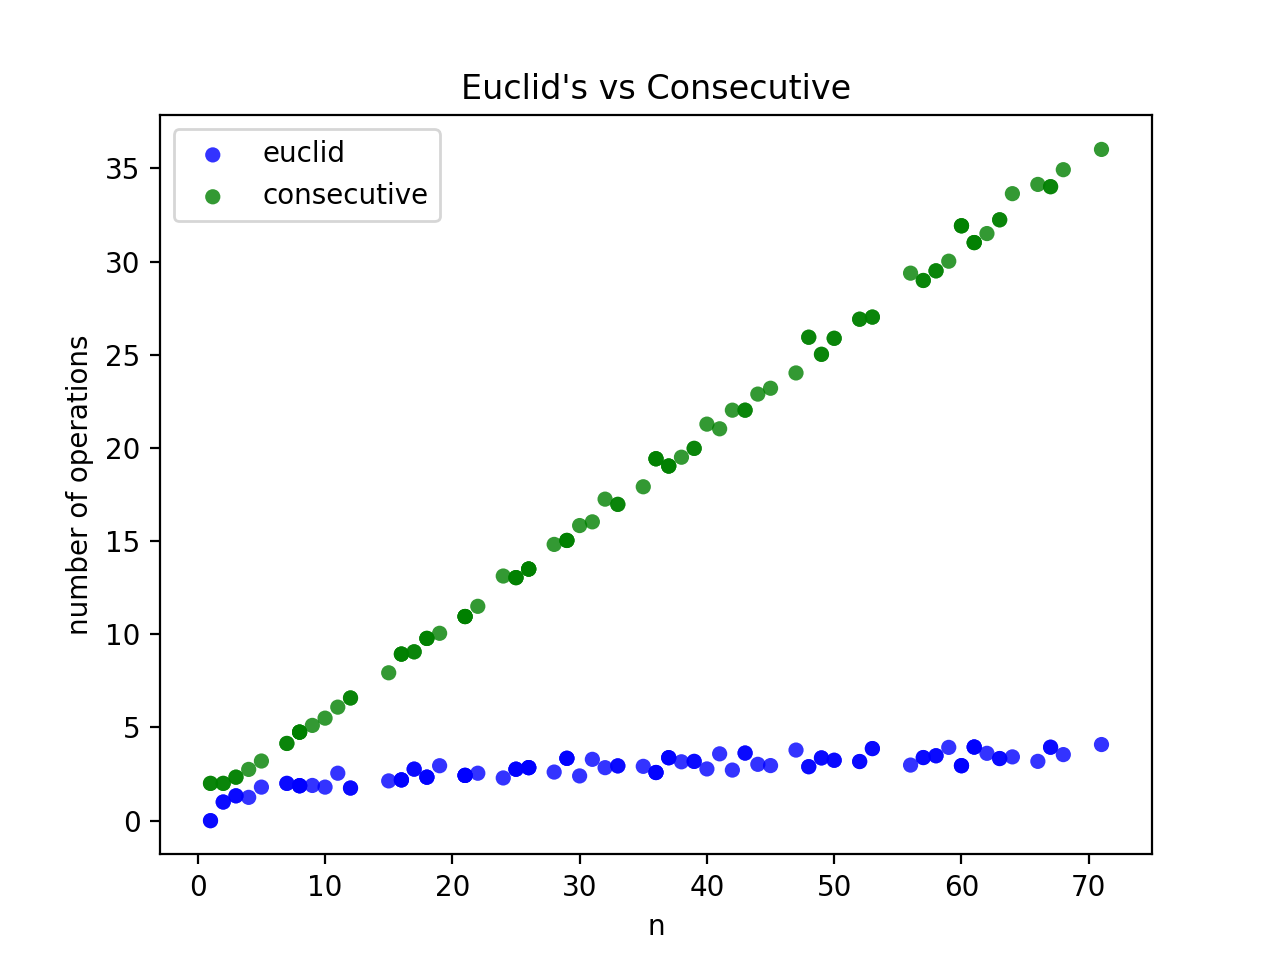
\includegraphics[scale=0.9]{task1.png}
		\linebreak
		\linebreak
		\linebreak
		\textbf{Euclid} $\theta$(logn)

		In the average case, Euclid's algorithm runs in $\theta$(logn) time and took less than 
		5 modulo divisions.
		
		\textbf{Consecutive Integer} $\theta$(n)

		The empirical testing shows the consecutive integer testing results to be nearly perfectly linear.

		\section{Task 2}

		\paragraph{Worst-case efficiency of Euclid's algorithm}
		The worst case for Euclid's algorithm occurs when two consecutive integers from the Fibonacci sequence are used as m and n. To test
		the efficiency, we generate 200 values for k between 1 and 20. k is an index in the Fibonacci sequence, where m = k + 1 and n = k.

		For example, based on the start of the Fibonacci sequence: [0, 1, 1, 2, 3, 5, 8, 13, 21, 34, 55]

		k = 5 => gcd(8, 5)

		k = 8 => gcd(34, 21)

		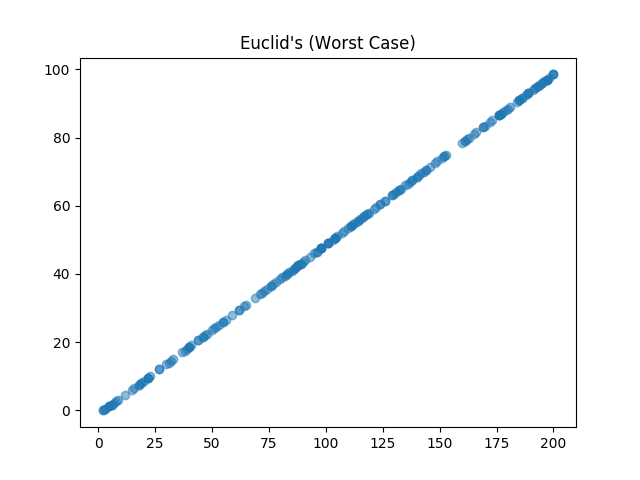
\includegraphics{task2}

		Because the gcd of two consecutive Fibonacci numbers is always 1, the complexity in the worst case for Euclid's algorithm
		is $\theta$(logn). We saw a trend that respresents a complexity of $\theta$(logn) in the average case as well, however the number
		of modulo divisions tended to be lower than how many were needed in the worst case.

		\paragraph{Time Analysis}

		We analyzed the time taken by Euclid's algorithm in the average and worst case by testing 5000 values. For the average case,
		we use values from 0 - 4999, and for the worst case we use consecutive Fibonacci numbers leading up until 
		position 5000 in the sequence.
		
		\textbf{Average Case:} 0.00000109137s

		\textbf{Worst Case: } 0.001714296s

		The average case input ran, on average, \textasciitilde{} 1000 times faster than the worst case input in our tests. This time analysis does not
		paint a picture of asymptotic complexity, and as the input size increases, the average time speedup will increase. For our fixed input size, we
		make the claim that the average case is \textasciitilde{}1000x faster than the worst case. This statement cannot be generalized to say the algorithm performs 1000x as fast for all
		average inputs as it does for worst case inputs.

		\paragraph{Upper Bound of k} We decided to set our upper bound of k to 1,000 because this is the point 
		at which the algorithm starts to take a few seconds to run. Python can handle larger values, but for the sake
		of this empirical analysis larger values are unnecessary.
		\pagebreak
		\section{Task 3}

		\paragraph{The "middle-school procedure"}
		To evaluate the complexity of the middle school method of calculating GCD, we generated 1000 pairs of random integers from 1 - 999 as m and n. When plotted, the results
		show that the middle school method is $\theta$(n).

		The algorithm works by finding all prime factors of both m and n using the Sieve of Eratosthenes. Once those factors are found,
		we generate the common factors in $\theta$(g), where g = max(|prime factors of m|, |prime factors of n|). We then multiply these common factors together
		to get gcd(m, n).

		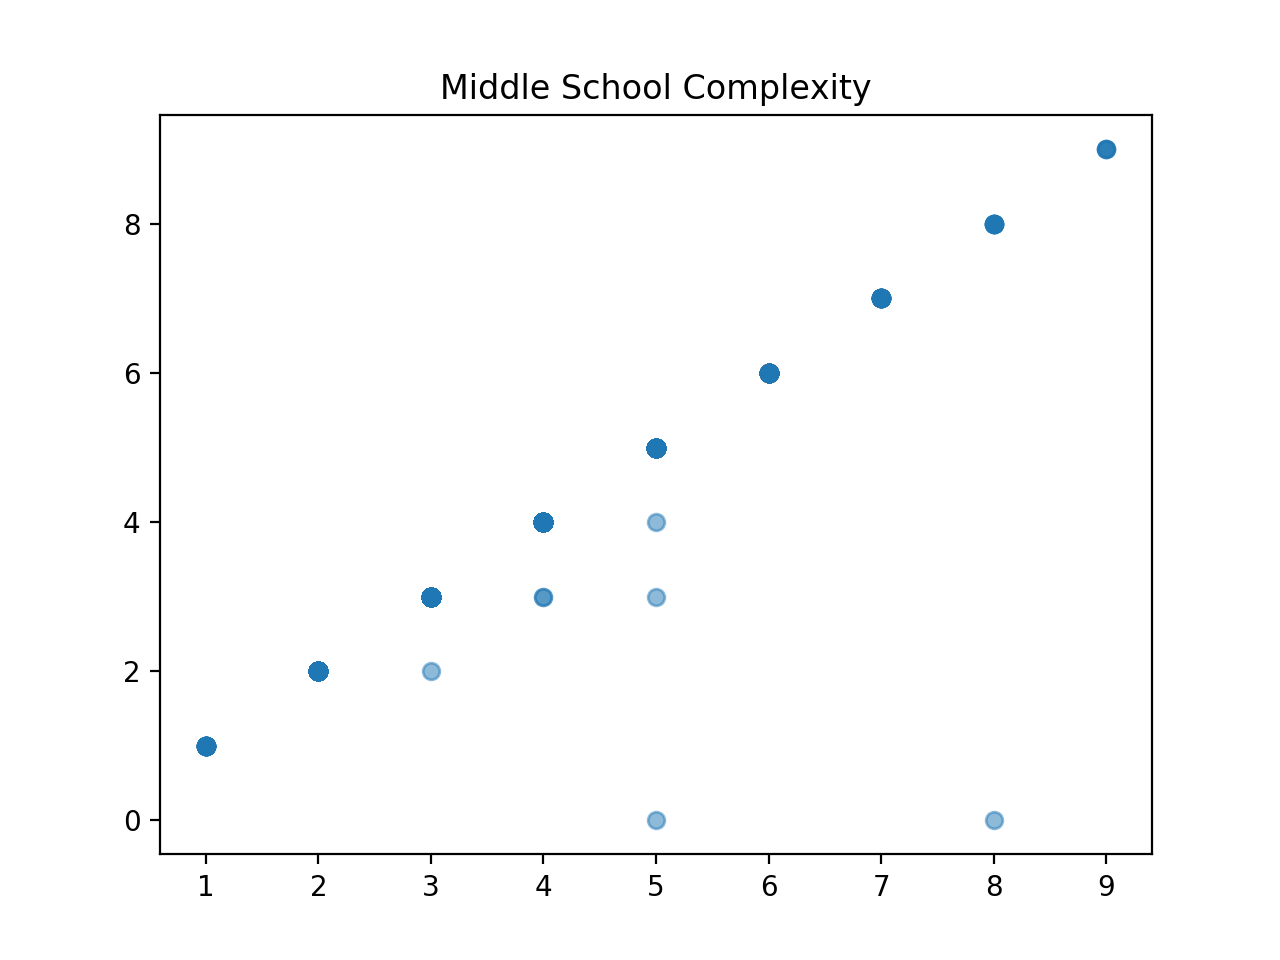
\includegraphics{task3}

		The evidence shows the complexity to be approximately linear, but there are some outliers where 
		both m and n had prime factors, but none were common and the gcd was determined to be 1. Darker dots on the
		scatter plot indicate where the majority of data points lie.

	\end{flushleft}
\end{document}